\documentclass{article}

\usepackage{amsmath}
\usepackage{amsthm}
\usepackage[utf8]{inputenc}
\usepackage{alltt}
\usepackage{amsfonts}
\usepackage{amssymb}
\usepackage{url}
\usepackage{subcaption}

\usepackage{pgf,tikz}
\usepackage{tkz-euclide}
\usetkzobj{all}

\theoremstyle{theorem}
\newtheorem{prop}{Proposition}[section]

\theoremstyle{theorem}
\newtheorem{thm}{Theorem}[section]

\newtheorem{remark}{Remark}[section]

\begin{document}

\title{Reinventing the wheel: designing wheels for staircases} \date{}
\author{
  Luís Pureza
}
\maketitle

\section{Introduction}

It is a well known fact that circular wheels are well suited to roll
over flat surfaces. Explaining why this is so is another matter, and
there is certainly a lot to find out if one starts investigating the
physics of motion in detail. There is, however, one convincing
argument that is simple to understand and doesn't require any physics:
if the wheel spins around an axle, a vehicle mounted on top of this
axle will always be at the same height from the road. Thus, if the
road is (approximately) flat, the vehicle will follow a straight line,
free of bumps and depressions. In a word, the journey could be
described as smooth.

Unfortunately, staircases are not flat and climbing or descending them
on circular wheels is anything but a smooth experience. This leads us
to wonder whether it would be possible to design wheels specialized
to roll over staircases while providing a comfortable ride. These
wheels could potentially be mounted on wheelchairs to help disabled
people, or used in small transportation vehicles in places where lifts
or ramps are unavailable.

In this document we propose to study the shape of wheels for
staircases. Perhaps surprisingly, we will find out that there is, for each staircase, an
infinite number of wheels matching our criteria for comfort and
smoothness, and we will develop an algorithm to design them all. Our
work follows from that of Hall and Wagon \cite{hall-wagon}, who
focused on the more general problem of designing wheels for roads of
arbitrary shape. They haven't, however, investigated in detail the
particular case of roads shaped like staircases.

The rest of this document is organised as follows. In section
\ref{sec:model} we express the problem of pairing roads and wheels
mathematically and derive a model to solve it. We then apply this
model, first in section \ref{sec:linear-roads} for the simpler case of
straight roads and then for staircases in section
\ref{sec:staircases}. This leads us to section \ref{sec:algorithm},
where we systematize all our findings and describe an algorithm to
build wheels for staircases, step by step. Then, in section
\ref{sec:proof-of-concept} we present a simulator that implements this
algorithm and is available online. Finally, we conclude with some
remarks regarding the feasibility of using these wheels in the real
world.

\section{Pairing roads and wheels }
\label{sec:model}

The question of designing wheels for arbitrary roads was posed by Hall
and Wagon in \cite{hall-wagon}, where they proved the equivalence to a
certain initial value problem. We begin by describing the mathematical
model they developed before applying it to the particular case of
staircases in subsequent sections.

Let us define a road as a two-dimensional curve given in parametric
coordinates

\begin{equation}
  \label{eq:road}
  (x, y) = (x(t), y(t)), \quad t \geq 0
\end{equation}

We can think of $t$ as the time since the motion started and $(x(t),
y(t))$ as the point of contact between the road and the wheel at time
$t$. Similarly, a wheel is a curve in polar form

\begin{equation}
  \label{eq:wheel}
  (r, \theta) = (r(\theta(t)), \theta(t)), \quad t \geq 0
\end{equation}
$(r(\theta(t)), \theta(t))$ represents the point on the border of the
wheel that will be in contact with the road after rolling for a time
$t$. Without loss of generality, we may assume the wheel starts
centred at the origin and the initial point of contact with the road
occurs right beneath it, that is,

\begin{equation}
  x(0)=0,\quad y(0)=-y_0 < 0, \quad \theta(0) = -\frac{\pi}{2}
\end{equation}

In order to be smooth, we require the motion to obbey the following constraints:\\

\noindent \textbf{No-bouncing} means the centre of the wheel must
travel along a linear path, without bumps or breaks. To simplify
calculations, we will presume this path is just the horizontal
axis. Consequently, the road is always below $y=0$ and the distance
between the centre of the wheel and the point of contact with the road
equals the height of the road. That is,

\begin{equation}
  \label{eq:no-bouncing}
  r(\theta(t)) = -y(t)
\end{equation}

\noindent \textbf{No-sliding} forces the wheel to roll over the road
without sliding. This means that the arc length between two points on
the wheel that touch the road at two different times must be the same
as the corresponding arc length on the road. Mathematically, this is
expressed as:

\begin{equation}
  \label{eq:no-sliding}
  \int_0^t{\sqrt{\left(\frac{dx}{dt}\right)^2+\left(\frac{dy}{dt}\right)^2}} dt = \int_{-\frac{\pi}{2}}^{\theta(t)}{\sqrt{r(\theta)^2+\left(\frac{dr}{d\theta}\right)^2}} d\theta
\end{equation}

It turns out that these two conditions simplify into a differential
equation that determines the wheel, as we shall see now.

Differentiating the no-sliding equation (\ref{eq:no-sliding}) with
respect to $t$ and squaring we get

\begin{equation}
  \label{after-squaring}
  \left(\frac{dx}{dt}\right)^2+\left(\frac{dy}{dt}\right)^2 = \left(r(\theta)^2+\left(\frac{dr}{d\theta}\right)^2\right)\left(\frac{d\theta}{dt}\right)^2
\end{equation}
But the no-bouncing condition (\ref{eq:no-bouncing}) tells us that

\begin{equation}
  \frac{dr}{dt} = \frac{dr}{d\theta}\frac{d\theta}{dt} = -\frac{dy}{dt} \quad \Leftrightarrow \quad \frac{dr}{d\theta} = -\frac{dy}{dt}\frac{dt}{d\theta}
\end{equation}
Substituting into (\ref{after-squaring}) and noting that we want
$\theta'(t)$ to be positive, we get

\begin{equation}
  \label{ivp}
  \frac{d\theta}{dt}=-\frac{1}{y(t)}\frac{dx}{dt}
\end{equation}
The solution to this differential equation subject to the initial
condition $\theta(0) = -\pi/2$ determines $\theta(t)$. If $\theta(t)$
is invertible, we can obtain $t(\theta)$ and use the no-bouncing
condition (\ref{eq:no-bouncing}) again to determine the radius of the
wheel at any angle $\theta$:

\begin{equation}
  r(\theta) = -y(t(\theta))
\end{equation}

Theoretically, if we can solve the initial value problem stated above
for a particular road, we get a wheel that fits it. In practice it is
not so simple, because the resulting wheel might not be closed (that
is, $r(\theta)$ is not periodic) or it might penetrate the road during
the motion.

\begin{remark}
  If the road is given by a cartesian equation $y=f(x)$, we can
  parametrize it by $x(t)=t$, $y(t)=f(t)$ and the initial value
  problem reduces to

  \begin{equation}
    \label{eq:ivp}
    \frac{d\theta}{dt}=-\frac{1}{y(t)}, \quad \theta(0) = -\pi/2
  \end{equation}
  All roads in the remaining of this text will be of this kind.
\end{remark}

% TODO: Confirm the penetration bit

\section{Wheels for straight roads}
\label{sec:linear-roads}

As a simple application of the model described above, let's confirm
our intuitive guess that circular wheels are perfect for flat roads.
\\

\noindent \textbf{The trivial example.} If the road is $y(x)=-y_0 $
where $y_0>0$ is constant, then the wheel is a circle of radius $y_0$.

\begin{proof}
  It is a direct consequence of the no-bouncing condition
  (\ref{eq:no-bouncing}).

  Let's confirm that this wheel does not slide. The distance travelled
  on the road after time $t$ is

 \begin{equation*}
   \int_0^t{\sqrt{\left(\frac{dx}{dt}\right)^2+\left(\frac{dy}{dt}\right)^2}}
   dt =
   \int_0^t{dt} = t
 \end{equation*}
 The initial value problem (\ref{eq:ivp}) gives
 $\theta(t)=\frac{1}{y_0}t-\frac{\pi}{2}$. Inverting we get
 $t(\theta)=\left(\theta+\pi/2\right)y_0$. But this is just the arc
 length of a circle of radius $y_0$ between angles $\theta(0)=-\pi/2$
 and $\theta(t)=\theta$, i.e., the distance covered by the wheel's
 border during the same amount of time $t$. Thus, this wheel obeys the
 no-sliding condition.
\end{proof}

The wheel becomes more complicated when the road has a slope. This is
because we force the centre of the wheel to move along the horizontal
axis, so its radius grows to infinity.

\begin{prop}
  \label{spiral-wheel}
  If the road is given by $y(x)=-mx-y_0$, where $m>0$ and $y_0>0$ are
  both constant, the corresponding wheel is given by
  $r(\theta)=y_0e^{m(\theta+\frac{\pi}{2})}$
\end{prop}

\begin{proof}
  Solving the initial value problem (\ref{eq:ivp}) we get

  \begin{equation}
    \theta(t)=\frac{\ln\left(\frac{mx}{y_0}+1\right)}{m}-\frac{\pi}{2}
  \end{equation}
  Inverting to get $t(\theta)$ gives

\begin{equation}
  t(\theta) = \frac{y_0}{m}\left(e^{m\left(\theta+\frac{\pi}{2}\right)}-1\right)
\end{equation}
Finally, substituting the above into the no-bouncing equation
(\ref{eq:no-bouncing}) results in

\begin{equation}
  r(\theta)=y_0e^{m\left(\theta+\frac{\pi}{2}\right)}
\end{equation}
which is the desired equation.
\end{proof}

\begin{remark}
  This wheel in Proposition \ref{spiral-wheel} is not closed, because
  the radius grows exponentially.
\end{remark}

The wheel above is a Bernoulli or logarithmic spiral, whose general
equation in polar coordinates is $r(\theta)=ae^{b\theta}$, where $a$
and $b$ are positive constants (the case $b=0$ degenerates into a
circle). Bernoulli spirals are equiangular, meaning that, at all
points, the angle between the radial and tangent lines remains
constant (see Figure \ref{fig:spiral}). This remarkable property is so
important for the remainder of our work that it merits its own
proposition and proof.

\begin{figure}
  \centering 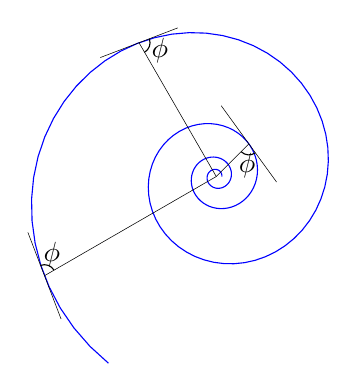
\begin{tikzpicture}[scale=0.7]

% Draw the spiral
\draw [blue, domain=0:1320, samples=200] plot ({1/10*exp(\x/360)*cos(\x)}, {1/10*exp(\x/360)*sin(\x)});

% WolframAlpha
% (1/10*exp(x/(2pi))*cos(x)+t, 1/10*exp(x/(2pi))*sin(x)+t*(sin(x)/((2pi))+cos(x))/(cos(x)/((2pi))-sin(x))) with x=pi/4+4pi, t=-5

\tkzDefPoint(0, 0){O}

% First tangent
\tkzDefPoint(0.09205325920345975, 1.2813330103113851){A1}
\tkzDefPoint(0.5920532592034597, 0.5920532592034602){A0}
\tkzDefPoint(1.0920532592034597, -0.09722649190446464){A2}
\tkzDrawLine[add=0 and 0](A1,A2)
\tkzDrawLine[add=0 and 0](O,A0)
\tkzMarkAngle[size=0.2](O,A0,A2)
\tkzLabelAngle[pos=0.4](O,A0,A2) {$\phi$}

% Second tangent
\tkzDefPoint(-1.9015812447263079, 2.2361089354271666){B1}
\tkzDefPoint(-1.4015812447263079, 2.427609926801592){B0}
\tkzDefPoint(-0.9015812447263079, 2.619110918176017){B2}
\tkzDrawLine[add=0.2 and 0.2](B1,B2)
\tkzDrawLine[add=0 and 0](O,B0)
\tkzMarkAngle[size=0.2](O,B0,B2)
\tkzLabelAngle[pos=0.4](O,B0,B2) {$\phi$}

% Third tangent
\tkzDefPoint(-3.4171128478167136, -1.0163801795332246){C1}
\tkzDefPoint(-3.117112847816714, -1.7996659417814145){C0}
\tkzDefPoint(-2.817112847816714, -2.5829517040296044){C2}
\tkzDrawLine[add=0 and 0](C1,C2)
\tkzDrawLine[add=0 and 0](O,C0)
\tkzMarkAngle[size=0.2](O,C0,C1)
\tkzLabelAngle[pos=0.4](O,C0,C1) {$\phi$}

\end{tikzpicture}

  \caption{Bernoulli spirals are equiangular}
  \label{fig:spiral}
\end{figure}


\begin{prop}
  \label{prop:equiangular}
  Bernoulli spirals are equiangular.
\end{prop}

\begin{proof}


  The parametric equation of the spiral,

\begin{equation}
  \left \lbrace
    \begin{array}{l}
      x(\theta)=r(\theta) \cos \theta \\
      y(\theta)=r(\theta) \sin \theta
    \end{array}
  \right. \quad
\end{equation}
allows us to find the derivative at $\left(x(\theta),
  y(\theta)\right)$:

\begin{equation}
  \frac{dy}{dx}
  =\frac{\frac{dy}{d\theta}}{\frac{dx}{d\theta}}
  =\frac{r'(\theta)\sin\theta+r(\theta)\cos\theta}{r'(\theta)\cos\theta-r(\theta)\sin\theta}
  =\frac{b\sin\theta+\cos\theta}{b\cos\theta-\sin\theta}
\end{equation}
where the last equality stems from the fact that $r'(\theta)=b
r(\theta)$.  Hence, the tangent vector at every point
$\left(x(\theta),y(\theta)\right)$ is

\begin{equation}
  \vec{T}=\left(1, \frac{b\sin\theta+\cos\theta}{b\cos\theta-\sin\theta}\right)
\end{equation}
while the radial unitary vector is just
$\hat{r}=(\cos\theta,\sin\theta)$.



Now, $\tan\alpha$, where $\alpha$ is the angle between the radial and
tangent vectors is just

\begin{equation}
  \tan\alpha
  =\frac{\sin\alpha}{\cos\alpha}
  =\frac{\left(\hat{r}\times\vec{T}\right)_z/\|\vec{T}\|}{\left(\hat{r}\cdot\vec{T}\right)/\|\vec{T}\|}
  =\frac{1}{b}
\end{equation}
$\left(\hat{r}\times\vec{T}\right)_z$ denotes the third component of
the cross product between $\hat{r}$ and $\vec{T}$ (extended into
$\mathbb{R}^3$ by setting $\hat{r}_z=\vec{T}_z=0$).

Finally, we see that $\tan\alpha$ is constant and thus $\alpha$ must
be constant as well.

\end{proof}

We shall now study what happens when the road is shaped like a
staircase.

\section{Finding a wheel for a staircase}
\label{sec:staircases}

\subsection{The first step}

To simplify, we will suppose the staircase is laid down in such a way
that the handrail is parallel to the horizontal axis, so that the
staircase looks more like a triangle wave. In this way the
(hypothetical) wheel will roll horizontally and we can apply the model
developed in section \ref{sec:model} to find it. Furthermore, let's
consider first the case of a staircase composed of a single step with
tread width $T$ and riser height $R$, as in Figure \ref{fig:step}.

\begin{figure}[h]
  \centering \begin{tikzpicture}[scale=0.03]
\tkzInit[ymin=-68,ymax=30,xmin=-80,xmax=40]

% Axis
\draw [->] (0,-68) -- (0,30) node[anchor=north east] {$y$};
\draw [->] (-180,0) -- (140,0) node[anchor=north east] {$x$};

% T=80, R=60, y0=-20
% x1=-64, x2=36
% The triangle's height is 48
\tkzDefPoint(-64,-68){A}
\tkzDefPoint(36,-68){B}
\tkzDefPoint(0,-20){C}
\tkzDrawLine[add=0 and 0, color=blue](A,C)
\tkzDrawLine[add=0 and 0, color=blue](C,B)

\tkzMarkRightAngle[size=4](B,C,A)

% T and R labels
\tkzLabelSegment[anchor=south east](A,C){$T$}
\tkzLabelSegment[anchor=south west](B,C){$R$}

% y0
\node at (0,-20) [right] {$-y_0$};
 
% x1 and x2
\draw [|-|, domain=-64:0] plot (\x, {-(20+48+6)});
\draw [-|, domain=0:36] plot (\x, {-(20+48+6)});

\node at (-32,-79) {$-x_1$};
\node at (18,-79) {$x_2$};

\tkzDefPoint(-100,-20){D}
\tkzDefPoint(-164,-68){E}
\tkzDrawLine[add=0 and 0, color=blue, dotted](A,D)
\tkzDrawLine[add=0 and 0, color=blue, dotted](E,D)

\tkzDefPoint(100,-20){F}
\tkzDefPoint(136,-68){G}
\tkzDrawLine[add=0 and 0, color=blue, dotted](B,F)
\tkzDrawLine[add=0 and 0, color=blue, dotted](F,G)

\end{tikzpicture}


  \caption{One step of the staircase}
  \label{fig:step}
\end{figure}

The equation of such a road is

\begin{equation}
  \label{eq:staircase}
  y(x)=
  \left \lbrace
    \begin{array}{ll}
      y_1(x) = mx-y_0, & x \in [x_1,0] \\
      y_2(x) = -\frac{1}{m}x-y_0, & x \in [0, x_2]
    \end{array}
  \right. \quad
\end{equation}
where $x_1<0$, $x_2>0$ and both $m$ and $y_0$ are positive constants.

It is not difficult to check that both line segments are perpendicular
to each other and that $y(x)$ is continuous at $x=0$. Moreover, a
simple application of the Pythagorean theorem shows that $m=R/T$, the
slope of the staircase.

To find a wheel for this road, we will apply Proposition
\ref{spiral-wheel} to both branches of $y(x)$. This gives the polar
curve

\begin{equation}
  \label{eq:petal}
  r(\theta)=
  \left \lbrace
    \begin{array}{ll}
      r_1(\theta) = y_0e^{-m\left(\theta+\frac{\pi}{2}\right)}, & \theta \in \left[-\frac{\pi}{2}-\theta_1,-\frac{\pi}{2}\right] \\
      r_2(\theta) = y_0e^{\frac{1}{m}\left(\theta+\frac{\pi}{2}\right)}, & \theta \in \left[-\frac{\pi}{2}, -\frac{\pi}{2}+\theta_2\right]
    \end{array}
  \right. \quad
\end{equation}
for some unknown $\theta_1$ and $\theta_2$.

We see that this curve is made up of two pieces of Bernoulli spirals
glued together. Because the spiral $r_1$ is tangent to $y_1$ at $x=0$
and $r_2$ is tangent to $y_2$ at the same location, we conclude that
both spirals intersect at an angle of $\pi/2$ and the curve fits the
road at the edge of the step (see Figure \ref{fig:petal}). Hence,
$r(\theta)$ is the wheel we were looking for.

\begin{figure}[h]
  \centering 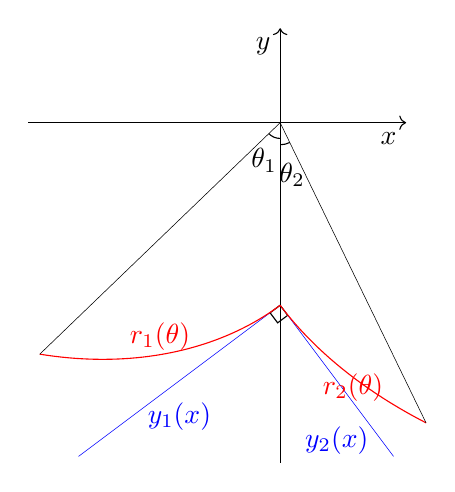
\begin{tikzpicture}[scale=0.04]

\tkzDefPoint(0, 0){O}

% Axis
\draw [->] (0,-108) -- (0,30) node[anchor=north east] {$y$};
\draw [->] (-80,0) -- (40,0) node[anchor=north east] {$x$};

% Draw the triangle
% T=80, R=60, y0=-20
% x1=-64, x2=36
% The triangle's height is 48
\tkzDefPoint(-64,-57.97570970504798-48){A}
\tkzDefPoint(36,-57.97570970504798-48){B}
\tkzDefPoint(0,-57.97570970504798){C}
\tkzDrawLine[add=0 and 0, color=blue](A,C)
\tkzLabelSegment[below=1ex, color=blue](A,C){$y_1(x)$}
\tkzDrawLine[add=0 and 0, color=blue](C,B)
\tkzLabelSegment[below=3ex, color=blue](C,B){$y_2(x)$}

\tkzMarkRightAngle[size=4](B,C,A)


% Draw the first petal
% y0:  57.97570970504798
% θ1 46.07999999999999
% θ2 25.919999999999998
\draw [red, domain=-(90+46.07999999999999):-90, samples=45]   plot ({57.97570970504798*exp(-(60/80)*(\x+90)/180*pi)*cos(\x)}, {57.97570970504798*exp(-(60/80)*(\x+90)/180*pi)*sin(\x)});
\draw [red, domain=-90:-(90-25.919999999999998), samples=25]  plot ({57.97570970504798*exp(+(80/60)*(\x+90)/180*pi)*cos(\x)}, {57.97570970504798*exp(+(80/60)*(\x+90)/180*pi)*sin(\x)});

% θ1
\tkzDefPoint(-76.33526011944696, -73.5104013727647){R1}
\tkzDrawLine[add=0 and 0](O, R1)
\tkzMarkAngle[size=5](R1,O,C)
\tkzLabelAngle[pos=13](R1,O,C) {$\theta_1$}

% θ2
\tkzDefPoint(46.323653594098744, -95.31510984719337){R2}
\tkzDrawLine[add=0 and 0](O, R2)
\tkzMarkAngle[size=7](C,O,R2)
\tkzLabelAngle[pos=17](C,O,R2) {$\theta_2$}

\tkzLabelSegment[below=-1.4ex, color=red](C,R1){$r_1(\theta)$}
\tkzLabelSegment[color=red](C,R2){$r_2(\theta)$}
\end{tikzpicture}



  \caption{The wheel for the first step}
  \label{fig:petal}
\end{figure}

To find the angles $\theta_1$ and $\theta_2$ we can apply the
no-sliding constraint (\ref{eq:no-sliding}), which reduces to

\begin{equation}
  \begin{array}{c}
    \displaystyle T=\int^{-\frac{\pi}{2}}_{-\frac{\pi}{2}-\theta_1}r_1(\theta)\sqrt{1+m^2}
    \,d\theta\\
    \\
    \displaystyle R=\int^{-\frac{\pi}{2}+\theta_2}_{-\frac{\pi}{2}}r_2(\theta)\sqrt{1+\frac{1}{m^2}} \,d\theta
  \end{array}
\end{equation}
Solving for $\theta_1$ and $\theta_2$ one gets

\begin{equation}
  \label{eq:thetas}
  \begin{array}{c}
    \displaystyle
    \theta_1=\frac{1}{m}\ln\left(\frac{R}{y_0\sqrt{1+m^2}}+1\right) \\
    \\
    \displaystyle \theta_2=m\ln\left(\frac{R}{y_0\sqrt{1+m^2}}+1\right)
  \end{array}
\end{equation}


\subsection{Completing the wheel}

Our strategy to build a wheel for a staircase with multiple steps will
be to stitch together multiple single-step wheels constructed in the
previous section, so that $r(\theta)$ becomes a periodic function of
period $\theta_1+\theta_2$. For reasons that will become apparent
soon, we will call these ``single-step wheels'' by \emph{petals} from
now on.

Is this wheel able to roll over the staircase? To show that it is, we
must prove some of its properties.

First, the wheel must be continuous at the point where two petals
intersect. That is, the radius at the rightmost point of a petal must
be equal to the radius at the leftmost point of the next one.

\begin{prop}
  The wheel is continuous at the point where two petals meet.
\end{prop}

\begin{proof}
  Simple calculations show that

  \begin{equation}
    r_1\left(-\frac{\pi}{2}-\theta_1\right)=r_2\left(-\frac{\pi}{2}+\theta_2\right)=\frac{R}{\sqrt{1+m^2}}+y_0
  \end{equation}
\end{proof}

Second, because two consecutive steps meet at an angle of $\pi/2$,
petals must intersect at the same angle, so that the wheel fits the
road. Coincidentally, this is the case.

\begin{prop}
  Petals intersect at an angle of $\pi/2$.
\end{prop}

\begin{proof}
  For this proof, we will refer to Figure
  \ref{fig:complete-wheel}. All the angles labelled $\alpha$ in this
  figure are congruent, due to the equiangular property of Bernoulli
  spirals proved in Proposition \ref{prop:equiangular}, and the same
  holds for the angles labelled $\beta$. But we already showed above
  that the two spirals that make up one petal intersect each other
  perpendicularly. Thus, $\alpha+\beta=\pi/2$, which concludes the
  proof.
\end{proof}

\begin{figure}[h]
  \centering 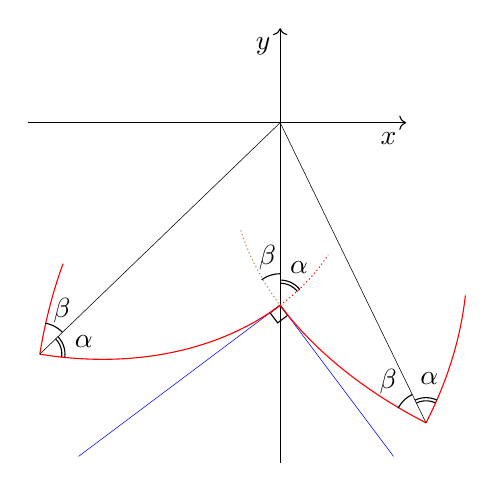
\begin{tikzpicture}[scale=0.04]

\tkzDefPoint(0, 0){O}

% Axis
\draw [->] (0,-108) -- (0,30) node[anchor=north east] {$y$};
\draw [->] (-80,0) -- (40,0) node[anchor=north east] {$x$};

% Draw the triangle
% T=80, R=60, y0=-20
% x1=-64, x2=36
% The triangle's height is 48
\tkzDefPoint(-64,-57.97570970504798-48){A}
\tkzDefPoint(36,-57.97570970504798-48){B}
\tkzDefPoint(0,-57.97570970504798){C}
\tkzDrawLine[add=0 and 0, color=blue](A,C)
\tkzDrawLine[add=0 and 0, color=blue](C,B)

\tkzMarkRightAngle[size=4](B,C,A)

% Draw the first petal
% y0:  57.97570970504798
% θ1 46.07999999999999
% θ2 25.919999999999998
\draw [red, domain=-(90+46.07999999999999):-90, samples=45]   plot ({57.97570970504798*exp(-(60/80)*(\x+90)/180*pi)*cos(\x)}, {57.97570970504798*exp(-(60/80)*(\x+90)/180*pi)*sin(\x)});
\draw [red, domain=-90:-(90-25.919999999999998), samples=25]  plot ({57.97570970504798*exp(+(80/60)*(\x+90)/180*pi)*cos(\x)}, {57.97570970504798*exp(+(80/60)*(\x+90)/180*pi)*sin(\x)});


\draw [red, domain=-(90+46.07999999999999)+72:-90+72-25, samples=45]   plot ({57.97570970504798*exp(-(60/80)*(\x+90-72)/180*pi)*cos(\x)}, {57.97570970504798*exp(-(60/80)*(\x+90-72)/180*pi)*sin(\x)});

\draw [red, domain=-90-72+15:-(90-25.919999999999998)-72, samples=25]  plot ({57.97570970504798*exp(+(80/60)*(\x+90+72)/180*pi)*cos(\x)}, {57.97570970504798*exp(+(80/60)*(\x+90+72)/180*pi)*sin(\x)});

\draw [red, densely dotted, domain=-90:-90+20, samples=45]   plot ({57.97570970504798*exp(-(60/80)*(\x+90)/180*pi)*cos(\x)}, {57.97570970504798*exp(-(60/80)*(\x+90)/180*pi)*sin(\x)});
\draw [brown, densely dotted, domain=-90-20:-90, samples=25]  plot ({57.97570970504798*exp(+(80/60)*(\x+90)/180*pi)*cos(\x)}, {57.97570970504798*exp(+(80/60)*(\x+90)/180*pi)*sin(\x)});


% θ1
\tkzDefPoint(-76.33526011944696, -73.5104013727647){R1}
\tkzDrawLine[add=0 and 0](O, R1)


% θ2
\tkzDefPoint(46.323653594098744, -95.31510984719337){R2}
\tkzDrawLine[add=0 and 0](O, R2)

% y+73.5104013727647 = 73.5104013727647/76.33526011944696(x+76.33526011944696)

% α1
\draw [domain=-7.5:-7.5+51.42] plot ({-76.33526011944696+8*cos(\x)},{-73.5104013727647+8*sin(\x)});
\draw [domain=-7.5:-7.5+51.42] plot ({-76.33526011944696+7*cos(\x)}, {-73.5104013727647+7*sin(\x)});
\node at (-76.33526011944696+14, -73.5104013727647+4) {$\alpha$};

\draw [domain=90-51.42:90] plot ({0+8*cos(\x)},{-57.97570970504798+8*sin(\x)});
\draw [domain=90-51.42:90] plot ({0+7*cos(\x)}, {-57.97570970504798+7*sin(\x)});
\node at (0+6, -57.9757097050479+12) {$\alpha$};


\draw [domain=-7.5+51.42:-7.5+51.42+36] plot ({-76.33526011944696+10*cos(\x)},{-73.5104013727647+10*sin(\x)});
\node at (-76.33526011944696+7, -73.5104013727647+14) {$\beta$};

%  y+95.31510984719337 = 95.31510984719337/46.323653594098744(x-46.323653594098744)

% α2
\draw [domain=90+25.92:90+25.92+36] plot ({46.323653594098744+10*cos(\x)}, {-95.31510984719337+10*sin(\x)});
\node at (46.323653594098744-12, -95.31510984719337+13) {$\beta$};

\draw [domain=90:90+36] plot ({0+10*cos(\x)}, {-57.97570970504798+10*sin(\x)});
\node at (0-4, -57.9757097050479+15) {$\beta$};


\draw [domain=90+25.92:90+25.92-51.42] plot
({46.323653594098744+8*cos(\x)}, {-95.31510984719337+8*sin(\x)});
\draw [domain=90+25.92:90+25.92-51.42] plot ({46.323653594098744+7*cos(\x)}, {-95.31510984719337+7*sin(\x)});
\node at (46.323653594098744+1, -95.31510984719337+14) {$\alpha$};
\end{tikzpicture}


  \caption{Two petals meet at an angle of $\pi/2$}
  \label{fig:complete-wheel}
\end{figure}


Finally, we must show the wheel is closed, so that it returns to the
initial position after one complete revolution. This basically amounts
to saying that we want $r(\theta)$ to be periodic of period
$2\pi$. But we already know that $r(\theta)$ is periodic of period
$\theta_1+\theta_2$, so the road will be closed if $2\pi$ is a
multiple of $\theta_1+\theta_2$. As the next proposition shows, we can
make this happen by varying the height of the wheel.

\begin{prop}
  Suppose we create a wheel as described with $N$ petals. The wheel is
  closed if and only if

  \begin{equation}
    \label{eq:y0}
    y_0=\frac{R}{\sqrt{1+m^2}\left(e^{\frac{2\pi m}{N(1+m^2)}}-1\right)}
  \end{equation}

\end{prop}

\begin{proof}
  Suppose the wheel is closed. Then, using the formulas
  (\ref{eq:thetas}) for $\theta_1$ and $\theta_2$ we get

  \begin{equation}
    \begin{array}{lcl}
      \theta_1+\theta_2=\frac{2\pi}{N} & \Leftrightarrow &
      \frac{m^2+1}{m}
      \ln\left(\frac{R}{y_0\sqrt{1+m^2}}+1\right)=\frac{2\pi}{N} \\
      & \Leftrightarrow
      & y_0=\frac{R}{\sqrt{1+m^2}\left(e^{\frac{2\pi
              m}{N(1+m^2)}}-1\right)}
    \end{array}
  \end{equation}
  The converse follows in the opposite direction.
\end{proof}

The proposition above allows us to conclude that, by varying the
height of the (imaginary) handrail where the centre of the wheel
passes, we can build a closed wheel with any number of petals. We have
just proved the following theorem:

\begin{thm}
  For every staircase, there is an infinite number of wheels, each
  with a different number of petals.
\end{thm}

\begin{figure}[h]
  \centering
  \begin{subfigure}[t]{.45\textwidth}
    \centering \input{fig-wheel3.tex}
    \caption{A wheel with 3 petals}
    \label{fig:wheel4}
  \end{subfigure}
  \begin{subfigure}[t]{.45\textwidth}
    \centering \begin{tikzpicture}[scale=0.7]

% Degrees to radians
\def\rad#1{(#1)/180*pi}

% Radians to degrees
\def\deg#1{(#1)*180/pi}

% r(θ)
\def \r#1#2{{(#1)*cos(#2)}, {(#1)*sin(#2)}}

\def \R{1.6}
\def \T{2.4}
\def \N{5}

\def \m{(\R/\T)}

% y0 in the paper
\def \y{(\R/(sqrt(\m*\m+1)*(exp((2 * pi * \m) / ((\m*\m+1) * \N)) - 1)))}

% θ1 in the paper
\def \theta {\deg{((1/\m) * ln(\R / (\y * sqrt(\m*\m+1)) + 1))}}

% θ2 in the paper
\def \phi {\deg{(\m * ln(\R / (\y * sqrt(\m*\m+1)) + 1))}}

% Increment in the angle of rotation of each petal
\def \dt{(360/\N)}

% Draw the N petals
\foreach \i in {1,...,\N}
{
  \draw [red, domain=-(90+\theta)+\dt*\i:-90+\dt*\i, samples=40] plot (\r{\y*exp(-\m*\rad{\x+90-\dt*\i})}{\x});
  \draw [red, domain=-90+\dt*\i:-(90-\phi)+\dt*\i, samples=40] plot (\r{\y*exp((1/\m)*\rad{\x+90-\dt*\i})}{\x});
}

% Draw the center
\tkzDefPoint(0, 0){O}
\tkzDrawPoint[color=red,fill=red](O)

\end{tikzpicture}


    \caption{A wheel with 5 petals}
    \label{fig:wheel5}
  \end{subfigure}
  \caption{Two wheels of different sizes for the same staircase}
  \label{fig:wheels}
\end{figure}

\section{An algorithm to build a wheel}
\label{sec:algorithm}

Suppose we are given a staircase with tread width $T$ and riser height
$R$. We can build a wheel for it made up of $N$ petals with the
following procedure:

\vspace*{0.15 cm}
\noindent \emph{\textbf{Step 1}} Find $m$, which is just the slope of
the staircase given by $R/T$.

\vspace*{0.15 cm}
\noindent \emph{\textbf{Step 2}} Compute $y_0$ according to
(\ref{eq:y0}):

  \begin{equation}
    y_0=\frac{R}{\sqrt{1+m^2}\left(e^{\frac{2\pi m}{N(1+m^2)}}-1\right)}
  \end{equation}

  \vspace*{0.15 cm}
  \noindent \emph{\textbf{Step 3}} Determine the angles $\theta_1$ and
  $\theta_2$ given by (\ref{eq:thetas}), i.e.,
  \begin{equation}
    \begin{array}{c}
      \displaystyle
      \theta_1=\frac{1}{m}\ln\left(\frac{R}{y_0\sqrt{1+m^2}}+1\right) \\
      \\
      \displaystyle \theta_2=m\ln\left(\frac{R}{y_0\sqrt{1+m^2}}+1\right)
    \end{array}
  \end{equation}

  \noindent \emph{\textbf{Step 4}} Build the first petal, that rolls
  over the first step, using the polar equation (\ref{eq:petal}), that
  is,

\begin{equation}
  r(\theta)=
  \left \lbrace
    \begin{array}{ll}
      r_1(\theta) = y_0e^{-m\left(\theta+\frac{\pi}{2}\right)}, & \theta \in \left[-\frac{\pi}{2}-\theta_1,-\frac{\pi}{2}\right] \\
      r_2(\theta) = y_0e^{\frac{1}{m}\left(\theta+\frac{\pi}{2}\right)}, & \theta \in \left[-\frac{\pi}{2}, -\frac{\pi}{2}+\theta_2\right]
    \end{array}
  \right. \quad
\end{equation}

\noindent \emph{\textbf{Step 5}} Complete the wheel by doing $N-1$
copies of the first petal, rotating them around the origin by an angle
of $2\pi k/N, \, k=1, 2, \cdots N-1$.

\hfill $\blacksquare$ \\

It is clear from the previous discussion that one could,
theoretically, build a wheelchair with two sets of wheels, one larger
at the back and one smaller up front, that is able climb or descend a
staircase while still providing a comfortable ride to its passenger.

\section{Proof of concept}
\label{sec:proof-of-concept}

We have implemented the algorithm developed in the previous section
into an interactive animation made available at
\cite{web-animation}. It works in any modern web browser, including
tablets and smartphones, without the need for any additional software.

This animation allows the user to enter the parameters for the
simulation, including the tread width $T$, the riser height $R$ and
the number of petals $N$ on the wheel. As soon as the user changes any
attribute, the wheel is rebuilt and it starts to descend the
staircase. The user can also choose to view a second wheel, in front
of the first, and select its size independently from the first.

To build the wheel we follow exactly the procedure outlined above. The
only complication is that, in order to animate the wheel, it was
necessary to calculate $\theta(t)$. However, retracing the steps in
Proposition \ref{spiral-wheel}, it is not difficult to verify that,
for the first step, $\theta(t)$ is given by

\begin{equation}
  \theta(t)=
  \left \lbrace
    \begin{array}{ll}
      \theta_1(t)=-\frac{\ln\left(1-\frac{m}{y_0}t\right)}{m}-\frac{\pi}{2},
      & t \in \left[x_1,0\right]
      \\
      \\
      \theta_2(t)=m\ln\left(\frac{1}{my_0}t+1\right)-\frac{\pi}{2},
      & t \in \left[0, x_2\right]
    \end{array}
  \right. \quad
\end{equation}

\begin{figure}[h]
  \centering
  \includegraphics[width=.9\linewidth]{fig-prototype.png}
  \caption{A screenshot of the working prototype showing two different
    wheels rolling over a staircase}
  \label{fig:prototype}
\end{figure}


\section{Conclusion}

In this document we have shown that it is possible to design wheels
properly suited to climb or descend stairs in such a way that any
vehicles attached to them will follow a linear path, free of
bumpiness, just like circular wheels do on flat surfaces. Moreover, we
have demonstrated that, for each stair, there are many different
wheels that can roll smoothly over it, all of them assembled from
segments of Bernoulli spirals. Finally, we have introduced an
algorithm to design these wheels, based on the dimensions of the
staircase and the desired size of the wheel, and implemented this
algorithm into a web application available online.

Unfortunately, as we have seen, there is no general purpose wheel that
works for all staircases. However, these wheels could still be useful
in some particular scenarios, such as public buildings or airplane
stairs, where the stairs have well known dimensions and wheels could
be built specifically for them. Further work needs to be done in order
to assess their applicability.

\begin{thebibliography}{10}

\bibitem{hall-wagon}Leon Hall and Stan Wagon, {\it Roads and Wheels},
  Mathematics Magazine, Vol. 65, No. 5 (Dec. 1992), 283--301.

\bibitem{leite}F. Silva Leite et al., {\it Wheels for staircases},
  Unpublished.

\bibitem{web-animation}Proof of concept,
  \url{http://pureza.github.io/app/} (Jun. 2015).

\end{thebibliography}


\end{document}
